\documentclass[11pt]{article}
\usepackage[margin=1in]{geometry}
\usepackage{newtxtext,newtxmath}
\usepackage[protrusion=true]{microtype}
\usepackage{booktabs,graphicx,xcolor,tikz,float}
\usetikzlibrary{positioning,arrows.meta}
\usepackage[font=normalsize,labelfont=bf,skip=3pt]{caption}
\usepackage[compact]{titlesec}
\usepackage[colorlinks=true,linkcolor=teal,citecolor=teal,urlcolor=teal]{hyperref}
\usepackage[authoryear,round]{natbib}
\titleformat{\section}{\normalsize\bfseries}{\thesection}{0.6em}{}
\titlespacing*{\section}{0pt}{1.0ex plus .2ex}{0.3ex}
\setlength{\parindent}{0pt}
\setlength{\parskip}{0.3em}
\setlength{\intextsep}{6pt plus 2pt}
\renewcommand{\arraystretch}{1.05}
\makeatletter\renewcommand\footnotesize{\@setfontsize\footnotesize\@xipt{13.6}}\makeatother
\setlength{\emergencystretch}{1em}
\setlength{\bibsep}{0pt}
\newcommand{\ci}[2]{\ensuremath{[#1,\,#2]}}
\definecolor{teal}{HTML}{0E6E6A}
\newcommand{\lref}[2]{\hyperref[#2]{#1~\ref*{#2}}}

\begin{document}
\begin{center}
{\large\bfseries PolyBridge: Option Prices Forecast Polymarket's Stock Contracts More Accurately Than Polymarket}\\[0.5ex]
{Theo Machado \quad Jacob Crainic}\\[0.1ex]
{Gator Quant Hacks 2026, Systematic Trading track}
\end{center}
{\centering\textbf{Abstract}\par}
Polymarket, a prediction market, lists contracts that pay \$1 if a stock closes above a stated price on a stated date. A spread of two listed call options on the same stock pays almost the same amount, so the options market also puts a price on this event. On 4,561 Polymarket stock contracts that no earlier test had used, the options price had squared forecast errors 11 percent smaller than the Polymarket price. The advantage is almost unchanged when the options price is read at the timestamp of the Polymarket price, but it falls to an amount we cannot tell apart from zero on the moments when the Polymarket price is less than 30 seconds old. None of the trading strategies built on the gap passed its registered test. A trade on contracts whose prices contradict the order of their deadlines turned positive only after a correction we made after seeing the results.

\section{Introduction}\label{sec:intro}
Polymarket and Kalshi are exchanges on which traders buy contracts that pay \$1 if an event occurs. A Polymarket stock contract pays \$1 if a stock closes above a stated price on a stated date and nothing otherwise, which makes it a digital option. A call option gives its holder the right to buy the stock at a fixed price, called the strike. Buying a call with a strike just below the stated price and selling one with a strike just above gives a call spread. Its payoff, divided by the gap between the strikes, matches the digital payoff unless the stock closes between the two strikes. The two markets therefore put a price on the same event, and we ask which of the two prices forecasts its outcome better. The answer matters to a market maker who quotes Polymarket's stock contracts and to a fund that reads these contracts as a signal.

We expect the options price to forecast better because option dealers update their quotes from liquid stock trading all day and offset their exposure in the stock, so an option quote moves within seconds of the stock. A Polymarket stock contract trades rarely and in small amounts, and its price can sit unchanged while the stock moves. The two prices can stay apart because the venues do not share collateral and money stays tied up until a contract pays out. The gaps are also worth only a few cents on small trades, so no large trader gains enough by closing them \citep{shleifer1997}. A competing explanation is that individual buyers in betting markets overpay for unlikely outcomes and underpay for likely ones, which pulls prices toward 50 percent \citep{snowberg2010}.

This reasoning predicts that the options price forecasts outcomes better and that its advantage is largest where the Polymarket price is oldest. It also predicts that thin markets break simple rules of their own, which we check on contracts about one news event with different deadlines in \lref{Section}{sec:lad}.

Our main contribution is a comparison, committed in advance, on 4,561 Polymarket stock contracts that no earlier test had used, in which the options price forecasts outcomes with 11 percent smaller squared errors than Polymarket's own price. We also compare Kalshi's index contracts, where the two prices are equally accurate within a margin set in advance, and we report every trading test, including the failures. PolyBridge, the trading system we release, labels each signal by whether it passed such a test and blocks orders that break its liquidity and loss limits.

Prediction-market prices measure the probability that traders assign to an event \citep{wolfers2004}. Option prices imply risk-neutral probabilities, which include compensation for bearing risk \citep{breeden1978} and the demand of investors who buy protection \citep{garleanu2009}, so we treat both prices as forecasts and score them against outcomes with the Brier score \citep{brier1950}.

\section{Data and method}\label{sec:data}
Polymarket's contract details, price histories and record of trades come from its public data service.\footnote{The repository holds the code, frozen contract lists, scored data and run logs: \url{https://github.com/theomachado05/polybridge}.} Option quotes and stock prices come from Massive, a market-data provider, and Kalshi prices come from Kalshi's public data service. A contract resolves when the venue declares whether the event occurred, and a print is a recorded trade. Our replays assume a fill only at a price that printed, which shows that someone traded there but not that the same size was still available to us.

At each comparison time we use the last value in Polymarket's per-minute price history at or before that time. Each test chooses its contracts by a fixed rule that reads contract details but no prices, uses only contracts that no earlier test had used, and was committed with its method before any price or outcome was fetched. The accuracy hypothesis came from discovery data, an earlier scan of contracts resolving from 15 August 2026 onward and two analyses of weekend reopenings, and the test reused that scan's direction, price filter, comparison times and option construction. The test contracts resolved between 21 November 2025 and 14 August 2026, before the discovery period, so they share no contract or outcome date with it but do not form the latest-dates holdout that the competition asks for. No stock contract has resolved since the discovery scan was committed on 3 October, so the forward test on contracts resolving from 5 October 2026 is the latest-dates holdout. All intervals are 95 percent intervals, except the 90 percent interval of the Kalshi equivalence test, and they resample whole resolution dates or events (\lref{Appendix}{app:rules}).

\section{Forecast accuracy}\label{sec:acc}
For each Polymarket contract asking whether a stock will close above \$$K$ on a given date, we took two listed calls on the same stock that expire on that date, with strikes $K_1 < K < K_2$. We then compared the two forecasts with the Brier score:
\begin{equation}
\hat p_{\mathrm{opt}} = e^{rT}\,\frac{C(K_1) - C(K_2)}{K_2 - K_1}, \qquad \mathrm{Brier} = \frac{1}{N}\sum_{i=1}^{N} \left(p_i - y_i\right)^2 .
\label{eq:main}
\end{equation}
Here $C(K)$ is the midpoint between the best bid and offer of the call with strike $K$, $r$ is a 4 percent interest rate and $T$ is the time to the close, so $\hat p_{\mathrm{opt}}$ is the cost of the call spread per dollar of its maximum payoff. Each option quote is at most 10 minutes old, and for 13.7 percent of moments a pair of strikes one step wider would move this probability by more than 5 percentage points. In the score, $p_i$ is either forecast at moment $i$ and $y_i$ is 1 if the contract paid out and 0 otherwise, so a lower score means smaller errors.

\begin{table}[H]
\centering
\caption{Brier scores on contracts that no earlier test used. The difference is the Polymarket score minus the options score, so a positive value favors options.}
\label{tab:acc}
\setlength{\tabcolsep}{3pt}
\begin{tabular}{@{}lrrccc@{}}
\toprule
Sample & Moments & Dates & Polymarket & Options & Difference [95\% interval] \\
\midrule
All test contracts & 7,111 & 89 & 0.0938 & 0.0831 & $+0.0108$ \ci{+0.0064}{+0.0158} \\
Options at Polymarket's timestamp & 7,107 & 89 & 0.0939 & 0.0836 & $+0.0103$ \ci{+0.0059}{+0.0153} \\
Polymarket price at most 30 s old & 669 & 15 & 0.0877 & 0.0865 & $+0.0012$ \ci{-0.0015}{+0.0052} \\
Trade within 10 minutes & 1,017 & 88 & 0.1101 & 0.1067 & $+0.0034$ \ci{+0.0004}{+0.0069} \\
\bottomrule
\end{tabular}
\end{table}

The options forecast had squared errors 11 percent smaller than the Polymarket price (\lref{Table}{tab:acc}). The difference is positive for daily and weekly contracts, at both comparison times and in the latest fifth of test dates, and it stays above zero when both prices must lie between 2 and 98 percent or when the five most influential dates are removed (\lref{Appendix}{app:acc}). Checks chosen after the test, such as dropping strike-sensitive moments, keeping one moment per contract or resampling whole calendar months, also keep it above zero (\lref{Table}{tab:explore}).

The Polymarket price we observe is on average 27 seconds older than the option quote. Measuring the options price at the timestamp of the Polymarket price leaves a difference of 0.0103 on 7,107 of the 7,111 moments, so a mismatch in observation times does not produce the gap. This check keeps the moments fixed and changes only when the options price is read, and the timestamps do not show when the Polymarket quote last changed.

\begin{figure}[H]
\centering
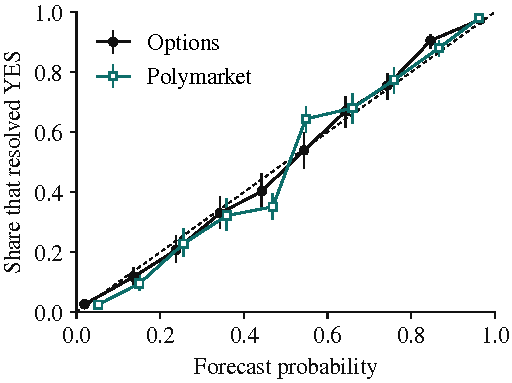
\includegraphics[scale=1]{fig/reliability.pdf}
\caption{Share of contracts that paid out, grouped by forecast, with the dashed line marking forecasts that match outcomes.}
\label{fig:rel}
\end{figure}

Compared with options, Polymarket prices sit closer to 50 percent (\lref{Figure}{fig:rel}), a pattern that buyers who overpay for unlikely outcomes would produce and that prices which have not caught up with the stock would also produce. On the 669 moments, from 15 dates, when the Polymarket price was at most 30 seconds old, the difference falls to 0.0012 with an interval that includes zero. That comparison selects a different sample rather than measuring the same moments differently, and all moments on its 15 dates give 0.0060, so it cannot separate the two explanations. Both prices add information in a joint regression, with the options forecast receiving the larger coefficient, and neither recalibration nor combining the two lowers the error of the raw options price by an amount distinguishable from zero.

On Kalshi's contracts on the S\&P 500 and Nasdaq-100, which professional market makers quote, the venue's prices matched options within a Brier margin of 0.003 set in advance. That comparison changes the underlying and the venue at once and selects contracts by lifetime trading volume, so it does not show why. A more accurate forecast is also not by itself a pricing error, because both prices carry compensation for risk, capital constraints and their own settlement rules. Crossing the options spread, the difference between the price to buy and the price to sell, costs a median of 2 cents and a mean of 7 cents per dollar of payoff. The mean gap is 6 cents, and no test traded it profitably at posted prices, so the options price is a candidate reference for quoting Polymarket's stock contracts that the forward test measures, rather than a strategy we have tested.

\section{Date ladders}\label{sec:lad}
Thin markets can also break their own logic, and Polymarket's date ladders allow a test of this that needs no outside price. A date ladder is a set of contracts on one news event with different deadlines, such as ``X happens by 15 January'' and ``X happens by 16 January'', and the earlier contract can never be worth more because it pays only if the later one pays too. When it trades above the later one, the replay buys NO on the earlier contract and YES on the later one. If the event happens before the first deadline or never, one of the two positions pays \$1, and if it happens between the deadlines both pay, so a correctly matched pair held to resolution cannot lose.

A text rule matched the written terms of 680 of 861 new pairs, and the replay entered when both contracts printed within 60 seconds at a gap larger than both fees plus one cent per contract. It traded the smaller print size, up to 100 contracts, and held both positions to resolution.

\begin{table}[H]
\centering
\caption{Ladder replay on new pairs, after fees, in cents per \$1 contract, with the 39 trades on unresolved markets valued at their guaranteed minimum.}
\label{tab:lad}
\begin{tabular}{lcccc}
\toprule
Version & Trades & Dates & Cents per trade [95\% interval] & Losing trades \\
\midrule
As registered & 650 & 221 & $+2.47$ \ci{-1.14}{+6.26} & 74 \\
Years corrected after the test & 562 & 211 & $+8.82$ \ci{+6.73}{+11.13} & 0 \\
\bottomrule
\end{tabular}
\end{table}

As registered, the replay found no reliable profit, and all 74 losing trades came from ladders whose deadlines the rule assigned to the wrong year. In a contract listed in March 2026, ``by December 31'' means December 2026, but the rule read December 2025 and so reversed the order of the two contracts. The correction reads each year from the listing date, and because we made it after seeing the losing trades, the corrected result is exploratory until the forward test from 5 October. Corrected, the replay has no losing trade and earned \$1,480 over its year of data. Of that amount, \$530 was the gap locked in at entry, and the rest came from 30 trades in which the event fell between the deadlines. Removing the 58 trades smaller than Polymarket's minimum order of 5 contracts leaves $+9.24$ cents per trade (\lref{Appendix}{app:lad}).

\section{Other trading tests}\label{sec:fail}
We ran about 40 tests under the method of \lref{Section}{sec:data}, and none of the 14 weekend and cross-venue strategies passed its registered rule, some because the effect was absent and some because too few markets qualified (Appendices~\hyperref[app:fail]{D} and~\hyperref[app:all]{F}).\footnote{Our study of company event filings (Form 8-K) for the Massive sponsor challenge is a \href{https://github.com/theomachado05/polybridge/blob/main/note/WRITEUP.md}{separate two-page report}.} The strongest lead was tickets that pay if a stock touches a price by a date. In earlier data, selling tickets priced at least 5 cents above an options-implied chance of a touch earned about 22 cents per contract, but on new markets only 32 contracts in 4 events qualified, against the 15 events the test required. Part of that premium is payment for exposure to the stock, because seller returns fell 2.3 cents per contract for each 1 percent the stock moved toward its target (\lref{Appendix}{app:touch}).

\section{Risk management and capital}\label{sec:risk}
PolyBridge, the system we built, connects each order to the evidence status of its signal, a person's approval and risk checks written in code (\lref{Figure}{fig:sys}). An order on a market that has not passed a committed test needs an explicit acknowledgment on top of that approval, and the trading library rejects any order when quotes are out of date, the market is closed, the spread is too wide or the book is too shallow. The library also limits position size, the dollar value of positions, the daily loss and the loss from the peak. Orders on Polymarket may not exceed half of what is offered within 2 cents of the best price, total exposure may not exceed half of the account, and exposure to one event may not exceed a fifth. The live recorder parses each Polymarket message and makes its decision in a median 3.4 millionths of a second, not counting network time.

\begin{figure}[H]
\centering
\begin{tikzpicture}[font=\normalsize, node distance=2.2mm,
  box/.style={draw, line width=0.5pt, align=center, inner sep=2pt, minimum height=9mm, text width=23.5mm},
  arr/.style={-{Latex[length=1.8mm]}, line width=0.5pt}]
\node[box] (src) {Market and option data};
\node[box, right=of src] (rec) {Order-book recorder};
\node[box, right=of rec] (det) {C++ signals};
\node[box, right=of det, draw=teal, line width=0.9pt] (gate) {Evidence check};
\node[box, right=of gate] (app) {Approval and risk limits};
\node[box, right=of app] (brk) {Paper broker account};
\node[box, below=2mm of gate, minimum height=6mm, text width=30mm] (res) {Committed tests};
\draw[arr] (src) -- (rec);
\draw[arr] (rec) -- (det);
\draw[arr] (det) -- (gate);
\draw[arr] (gate) -- (app);
\draw[arr] (app) -- (brk);
\draw[arr] (res) -- (gate);
\end{tikzpicture}
\caption{Every order needs a person's approval and passes the risk checks, and an order whose market has not passed a committed test also needs an explicit acknowledgment.}
\label{fig:sys}
\end{figure}

The ladder and ticket rules below are a plan that code must enforce before either trade goes live, starting with a person checking the written rules and deadline years of every ladder pair before its first order. If the second leg does not fill within 60 seconds, the system cancels it and closes the first leg with a limit order, and a person takes over if that order does not fill. Reaching the daily loss threshold blocks new orders and calls a person, but a fast move or a failed exit can still produce a larger loss. Money tied up until one resolution date is limited to a fifth of the account, and a quarter of ladder capital stays in cash. Sold touch tickets on one stock lose together, so the payout owed on any one stock is capped at 5 percent of the account, which is the most a stock that reaches its target can cost before the premium collected. At the historical sensitivity, a 5 percent move toward the target costs about 0.6 percent of the account, and sudden moves can cost more.

\begin{table}[H]
\centering
\caption{Capacity at the 100-contract cap and in books recorded on 3 October, with a median spread of 9 cents.}
\label{tab:cap}
\begin{tabular}{lc}
\toprule
Quantity & Value \\
\midrule
Ladder replay profit on new pairs over one year, assumed fills & \$1,480 \\
Ladder capital tied up at most & about \$3,000 \\
Polymarket stock book depth within 2 cents, quartiles & 210 / 570 / 1,013 contracts \\
Gross gap, not revenue: 6 cents on half the depth of 200 markets & about \$3,400 \\
\bottomrule
\end{tabular}
\end{table}

\section{Future work and conclusion}\label{sec:future}
Four tests, each committed with its rule for passing, begin on 5 October 2026 and compare the two forecasts with prices recorded at the same moment, run the corrected ladder rule on new ladders and the ticket rule on newly listed markets, and replace traded sizes with recorded order-book depth in every capacity estimate. On the stock contracts we tested, options forecast outcomes better than Polymarket's own price, and the open question is how much of that gap comes from Polymarket prices that had not yet caught up with the stock. If slow updating causes it, the gap should shrink when both prices are recorded just after a Polymarket quote changes, and if risk compensation or settlement rules cause it, the gap should persist. PolyBridge keeps this distinction in its rules, so a signal without a passed test reaches the broker only with a person's acknowledgment.

{
\begin{thebibliography}{6}\setlength{\itemsep}{0pt}\setlength{\parskip}{0pt}
\bibitem[Breeden and Litzenberger(1978)]{breeden1978} Breeden, D.~T. and Litzenberger, R.~H. (1978). Prices of state-contingent claims implicit in option prices. \emph{Journal of Business}, 51(4):621--651.
\bibitem[Brier(1950)]{brier1950} Brier, G.~W. (1950). Verification of forecasts expressed in terms of probability. \emph{Monthly Weather Review}, 78(1):1--3.
\bibitem[G\^arleanu et~al.(2009)]{garleanu2009} G\^arleanu, N., Pedersen, L.~H. and Poteshman, A.~M. (2009). Demand-based option pricing. \emph{Review of Financial Studies}, 22(10):4259--4299.
\bibitem[Shleifer and Vishny(1997)]{shleifer1997} Shleifer, A. and Vishny, R.~W. (1997). The limits of arbitrage. \emph{Journal of Finance}, 52(1):35--55.
\bibitem[Snowberg and Wolfers(2010)]{snowberg2010} Snowberg, E. and Wolfers, J. (2010). Explaining the favorite--long shot bias: Is it risk-love or misperceptions? \emph{Journal of Political Economy}, 118(4):723--746.
\bibitem[Wolfers and Zitzewitz(2004)]{wolfers2004} Wolfers, J. and Zitzewitz, E. (2004). Prediction markets. \emph{Journal of Economic Perspectives}, 18(2):107--126.
\end{thebibliography}}

\appendix
\section{Accuracy by subset}\label{app:acc}
\begin{figure}[H]
\centering
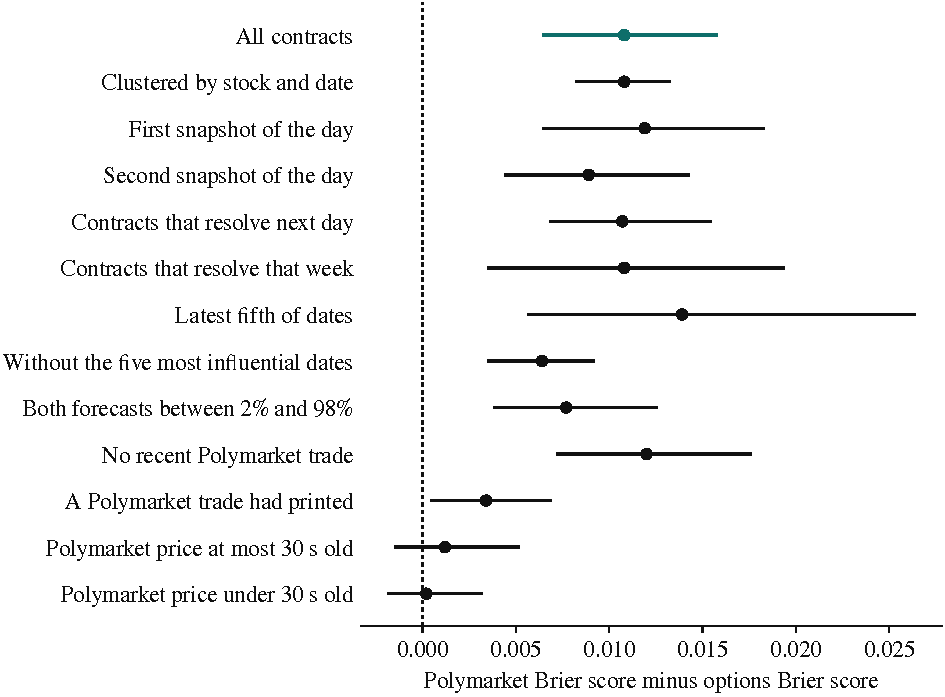
\includegraphics[scale=1]{fig/subsets.pdf}
\caption{Polymarket Brier score minus options Brier score by subset, with 95\% intervals, where values right of the dashed line favor options and the teal row is the primary result (numbers in Table~\ref{tab:subsets}).}
\label{fig:subsets}
\end{figure}
\begin{table}[H]
\centering
\caption{Polymarket minus options by subset, where positive values favor options and intervals resample resolution dates unless noted. ``Trade printed'' means a trade within 10 minutes before or after the comparison.}\label{tab:subsets}
\setlength{\tabcolsep}{2pt}
\begin{tabular}{lccc}
\toprule
Subset & Rows & Brier difference & Log-score difference \\
\midrule
All (primary) & 7,111 & $+0.0108$ \ci{+0.0064}{+0.0158} & $+0.0318$ \ci{+0.0170}{+0.0471} \\
Stock and date clusters & 7,111 & $+0.0108$ \ci{+0.0082}{+0.0133} & $+0.0318$ \ci{+0.0211}{+0.0407} \\
First snapshot & 4,404 & $+0.0119$ \ci{+0.0064}{+0.0183} & $+0.0332$ \ci{+0.0136}{+0.0530} \\
Second snapshot & 2,707 & $+0.0089$ \ci{+0.0044}{+0.0143} & $+0.0296$ \ci{+0.0167}{+0.0445} \\
Daily contracts & 3,501 & $+0.0107$ \ci{+0.0068}{+0.0155} & $+0.0330$ \ci{+0.0215}{+0.0466} \\
Weekly contracts & 3,610 & $+0.0108$ \ci{+0.0035}{+0.0194} & $+0.0306$ \ci{+0.0060}{+0.0562} \\
A Polymarket trade printed & 1,017 & $+0.0034$ \ci{+0.0004}{+0.0069} & $+0.0123$ \ci{+0.0027}{+0.0230} \\
No Polymarket trade printed & 6,094 & $+0.0120$ \ci{+0.0072}{+0.0176} & $+0.0351$ \ci{+0.0184}{+0.0519} \\
Latest 20\% of dates & 1,299 & $+0.0139$ \ci{+0.0056}{+0.0264} & \\
Without 5 most influential dates & 6,448 & $+0.0064$ \ci{+0.0035}{+0.0092} & \\
Both forecasts in 2\% to 98\% & 4,774 & $+0.0077$ \ci{+0.0038}{+0.0126} & \\
Polymarket price at most 30 s old & 669 & $+0.0012$ \ci{-0.0015}{+0.0052} & \\
Polymarket price under 30 s old & 608 & $+0.0002$ \ci{-0.0019}{+0.0032} & \\
\bottomrule
\end{tabular}
\end{table}
In a logistic regression of outcomes on both forecasts, with date-clustered intervals, the options coefficient is $0.85$ \ci{0.63}{1.07} and the Polymarket coefficient is $0.30$ \ci{0.15}{0.45}. Pooled over both series, the Kalshi index price matched options within the margin of $\pm0.003$ set in advance, with a 90\% interval of \ci{+0.0001}{+0.0025}, and the S\&P 500 series alone favored options by $0.0016$ \ci{+0.0003}{+0.0030}. The Kalshi rule kept the eight contracts of each event with the most lifetime volume, a field recorded after the comparison time.

\begin{table}[H]
\centering
\caption{Checks chosen after the test, on the same scored moments. Differences are a score minus the options Brier score, so positive values favor options, and intervals resample the cluster shown.}
\label{tab:explore}
\setlength{\tabcolsep}{3pt}
\begin{tabular}{lrrc}
\toprule
Check & Rows & Clusters & Difference [95\% interval] \\
\midrule
Registered result & 7,111 & 89 dates & $+0.0108$ \ci{+0.0064}{+0.0158} \\
Without strike-sensitive moments & 5,835 & 89 dates & $+0.0112$ \ci{+0.0068}{+0.0163} \\
Earliest moment per contract & 4,561 & 89 dates & $+0.0120$ \ci{+0.0065}{+0.0183} \\
Each stock and date weighted equally & 570 groups & 89 dates & $+0.0118$ \ci{+0.0075}{+0.0167} \\
Resampling calendar weeks & 7,111 & 35 weeks & $+0.0108$ \ci{+0.0060}{+0.0164} \\
Resampling four-week blocks & 7,111 & 11 blocks & $+0.0108$ \ci{+0.0052}{+0.0189} \\
All moments on the 30 s subset's dates & 1,186 & 15 dates & $+0.0060$ \ci{-0.0003}{+0.0152} \\
Older moments on those dates & 517 & 12 dates & $+0.0123$ \ci{+0.0005}{+0.0288} \\
Options at Polymarket's timestamp & 7,107 & 89 dates & $+0.0103$ \ci{+0.0059}{+0.0153} \\
Same, Polymarket price at most 30 s old & 669 & 15 dates & $+0.0011$ \ci{-0.0012}{+0.0045} \\
\midrule
Average of the two prices minus options & 7,111 & 89 dates & $+0.0023$ \ci{+0.0009}{+0.0039} \\
After 20 dates: Polymarket minus options & 5,179 & 69 dates & $+0.0076$ \ci{+0.0038}{+0.0120} \\
After 20 dates: recalibrated options & 5,179 & 69 dates & $+0.0009$ \ci{-0.0010}{+0.0035} \\
After 20 dates: combined minus options & 5,179 & 69 dates & $+0.0010$ \ci{-0.0008}{+0.0037} \\
\bottomrule
\end{tabular}
\end{table}
Recalibrated and combined forecasts come from logistic regressions fitted only on contracts whose outcomes were known before the first comparison time of each date, starting after the first 20 dates. The 20-date start, the model form and every check in this table were chosen after the registered test.

\section{Ladder details}\label{app:lad}
\begin{figure}[H]
\centering
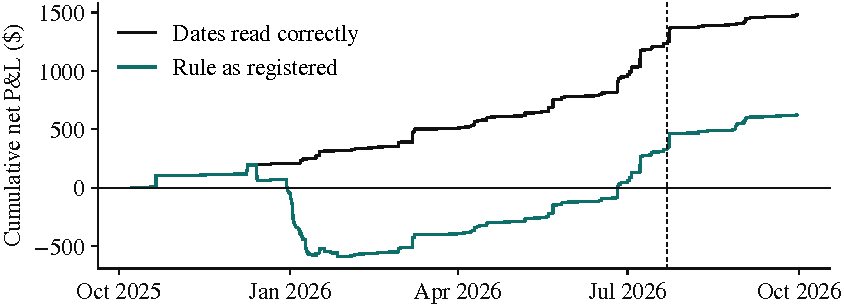
\includegraphics[scale=1]{fig/ladder.pdf}
\caption{Cumulative profit of the fresh ladder replay after fees, under the registered rule and with years corrected after the test. The dashed line marks the start of the period that an earlier study held out.}
\label{fig:lad}
\end{figure}
\begin{table}[H]
\centering
\caption{Rule check and replay on the pairs of the earlier study, whose data we had already seen, and on fresh pairs.}
\begin{tabular}{p{6.4cm}cc}
\toprule
 & Earlier pairs & Fresh pairs \\
\midrule
Pairs & 918 & 861 \\
Nested under the registered rule & 727 & 680 \\
Nested after the date correction & 720 & 676 \\
Excluded: written rules or source differ & 89 & 109 \\
Excluded: window starts at listing, later contract listed later & 102 & 70 \\
Excluded: no market record & 0 & 2 \\
Nested pairs removed by the date correction & 7 & 4 \\
Trades as registered & 691, $+5.16$ \ci{+2.31}{+8.30} & 650, $+2.47$ \ci{-1.14}{+6.26} \\
Trades after the date correction & 575, $+9.40$ \ci{+6.54}{+12.48} & 562, $+8.82$ \ci{+6.73}{+11.13} \\
Corrected, from 22 July 2026 & 48, $+8.27$ \ci{+1.88}{+16.77} & 102, $+9.20$ \ci{+4.86}{+14.01} \\
Profit per year at 100 contracts & \$1,818 & \$1,480 \\
\bottomrule
\end{tabular}
\end{table}
As registered, the fresh replay lost up to \$649 from its peak. The corrected profit of \$1,480 is 8.5 percent of the \$17,460 committed across all trades, while the most capital tied up at once was about \$3,000. The typical fresh trade was 19 contracts, and 58 trades were smaller than Polymarket's minimum order of 5 contracts, without which the corrected result is $+9.24$ cents \ci{+7.02}{+11.70}. Of the 98 violations that the earlier study confirmed with prints on both legs, 65 pass the 60-second rule, 19 fail it and 14 sit on pairs that are not nested. A scan of the 34 live ladders at 01:57 ET on 4 October found no violation after fees, and the median pair was 10.5 cents away from one.

\section{Ticket details}\label{app:touch}
\begin{figure}[H]
\centering
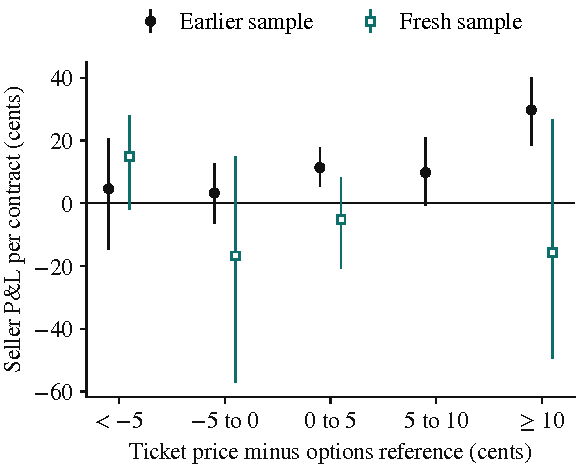
\includegraphics[scale=1]{fig/touch.pdf}
\caption{Seller profit by ticket price minus the options-implied chance of a touch, with 95\% intervals that resample events, where filled markers are earlier data, open markers are new markets, and buckets with fewer than three events are omitted.}
\end{figure}
The seven tickets that qualified in a larger secondary sample lost $15.4$ cents per contract on average, with an interval of \ci{-48.8}{+21.8}. Across 36 markets with a stock move, seller returns fell 2.3 cents for each 1\% move of the stock toward its target \ci{-4.56}{-0.05}. With its stock exposure offset by holding shares, which traders call delta hedging, the full seller book earned $+10.5$ cents \ci{-0.1}{+20.0} on 37 markets, one more than the regression because one market lacks a closing price for a holiday week.

\section{Tests that failed}\label{app:fail}
\begin{table}[H]
\centering
\begin{tabular}{p{7.6cm}p{7.0cm}}
\toprule
Test & Result \\
\midrule
8-K filings predict option mispricing (\href{https://github.com/theomachado05/polybridge/blob/main/note/WRITEUP.md}{separate report}) & Null in sample, reversed sign out of sample \\
Overnight Polymarket moves predict the open of SPY, an S\&P 500 index fund & Did not replicate on 10 new markets or 36 US macro markets \\
Polymarket adds to pre-market SPY & No: $-0.60$ basis points (hundredths of a percent) per point \ci{-2.64}{+1.44} at 08:00 \\
Trade Polymarket toward options after weekends & $-0.40$ cents per trade \ci{-4.68}{+3.74}, 402 trades \\
Overnight hedge on a long SPY book & Lost \$7,318 in sample, no trade out of sample \\
14 weekend and cross-venue studies & None passed its registered rule, some for lack of data \\
\bottomrule
\end{tabular}
\end{table}

\section{Test rules}\label{app:rules}
\textbf{Accuracy.} The options probability is the discount-adjusted price of a call spread around the strike divided by its width, from quotes at most 10 minutes old. The Polymarket price is the last value in its per-minute history at or before the comparison, at most 15 minutes old, and rows with a Polymarket price outside 2\% to 98\% are dropped. Polymarket settles on a 16:00 price published by a data provider, and options on the official closing price. The test needed both the Brier and the log-score intervals above zero, where the log score is the average of minus the logarithm of the probability a forecast gave to what happened.

\textbf{Ladders.} Two contracts are nested when their written rules match after the deadline is removed and they name one resolution source. The replay enters at the first moment both contracts print within 60 seconds at a gap that exceeds both fees plus one tick (one cent) per leg, sizes at the smaller print up to 100 contracts, and holds to resolution. The first run was voided after its diagnostics, which included the losing trades, showed that the trade data mapped some prints to the wrong outcome, and its output is archived in the repository. The pass rule needed a date-clustered interval above zero with at least 30 trades on 15 dates.

\textbf{Tickets.} The touch probability comes from two option quotes at 15:55 on the Friday before the ticket's first weekend, converted from the chance of closing above the price to the chance of touching it, assuming the stock has no expected trend. The rule sells the ticket at a printed bid when its price is at least 5 cents above that chance and holds it to resolution. The pass rule needed 30 markets in 15 events with an event-clustered interval above zero.

\section{All tests on one scale}\label{app:all}
\begin{figure}[H]
\centering
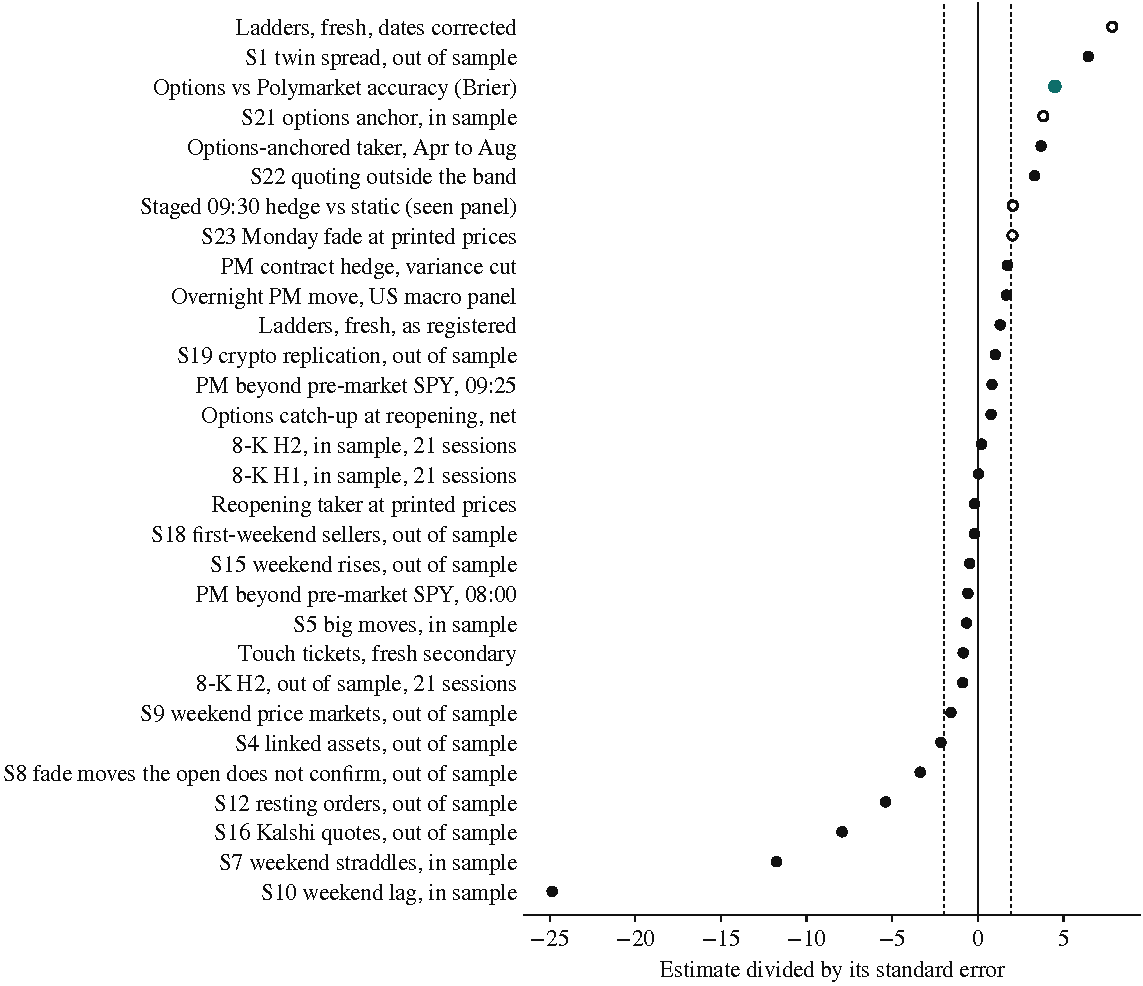
\includegraphics[width=\linewidth]{fig/search.pdf}
\caption{Each test's primary estimate divided by its standard error, taken from its 95\% interval, with dashed lines at $\pm1.96$. Teal marks the registered test that passed, open markers mark results corrected after the run or on data already seen, and filled markers mark tests that failed their own rule. Units differ across tests, so the figure compares strength of evidence and not economic value.}
\end{figure}


\end{document}
